\documentclass[10pt,a4paper]{article}
\usepackage[utf8]{inputenc}
\usepackage{amsmath}
\usepackage{amsfonts}
\usepackage{amssymb}
\usepackage{graphicx}
\author{Andrea Colarieti Tosti}
\title{Lineare Algebra Tutorium 8 Lösung}

\begin{document}
 \maketitle
 \newpage
 
 \section{Aufgabe 1}
 \subsection{i}
 Zu zeigen :
 \begin{enumerate}
 \item $H \neq \emptyset$
 \item $ u+v \in H , \; u,v \in H$
 \item $ \lambda u \in H, \; \lambda \in \mathbb{R}, \; u \in H $
 \item eine Menge von Vektoren $V \subseteq \mathbb{R}^3$ angeben, so dass U = span(V)
 \end{enumerate}
 \paragraph{1} $H \neq \emptyset$\\\\
 Sei $\phi$ eine lineare Abbildung $\phi: \mathbb{R}^3 \rightarrow H , x \mapsto v + x, \; v \in H, \; x \in U \subseteq \mathbb{R}^3 $\\
 $$ \phi(0,0,0) = v + (0,0,0) = v \in H $$
 Also ist H nicht leer.
 \paragraph{2} $ u+v \in H , \; u,v \in H$\\\\
 Seien $u,w \in H , \; v \in \mathbb{R}^3$ definiert wie folgt:\\
  $v=(v_1,v_2,v_3)$; $u=(u_1,u_2,u_3)+v$; $w=(w_1,w_2,w_3)+v$ mit $v_1,v_2,v_3 \in \mathbb{R}$ und   $(u_1,u_2,u_3)(w_1,w_2,w_3) \in U$ \\
  $$ u+ v = ((u_1,u_2,u_3)+(v_1,v_2,v_3))+((w_1,w_2,w_3)+(v_1,v_2,v_3))$$
  $$= (u_1+v_1,u_2+v_2,u_3+v_3)+(w_1+v_1,w_2+v_2,w_3+v_3) $$
  $$= (u_1+v_1+w_1+v_1,u_2+v_2+w_2+v_2,u_3+v_3+w_3+v_3)$$
  $$= (2v_1+u_1+w_1,2v_2+u_2+w_2,2v_3+u_3+w_3)$$
  $$= 2v+(u_1+w_1,2u_2+w_2,u_3+w_3) $$
  $$= 2v+(u_1+w_1,2u_2+w_2,u_3+w_3) $$
  $$\underbrace{2v}_{\in \mathbb{R}^3}+\underbrace{(u_1+w_1,2u_2+w_2,u_3+w_3)}_{\in U}$$
  Es handelt sich um einen Vektor der Form $v + u \in H$.
 \paragraph{3} $ \lambda u \in H, \; \lambda \in \mathbb{R}, \; u \in H $\\\\
 Sei $ u \in H $, $u:=(u_1,u_2,u_3)+v$; $v:=(v_1,v_2,v_3) \in\mathbb{R}$; $(u_1,u_2,u_3) \in U\subseteq \mathbb{R}^3$ und $\lambda \in \mathbb{R}$\\
 $$ \lambda u = \lambda ((u_1,u_2,u_3)+(v_1,v_2,v_3))= \lambda (u_1+v_1,u_2+v_2,u_3+v_3)$$
 $$ (\lambda (u_1+v_1),\lambda (u_2+v_2),\lambda (u_3+v_3))= \underbrace{\lambda v}_{\in \mathbb{R}^3} + \underbrace{\lambda u}_{\in U}$$
  Es handelt sich wieder um einen Vektor der Form $v + u \in H$.
  \paragraph{4}eine Menge von Vektoren $V \subseteq \mathbb{R}^3$ angeben, so dass U = span(V)\\\\
  $ V := \{(1,0,0)(0,1,0)(0,0,1)\} \\\Rightarrow span(V)=\{ \alpha(1,0,0),\beta(0,1,0),\gamma(0,0,1) \} = U \subseteq \mathbb{R}^3$ mit $ \alpha, \beta, \gamma \in \mathbb{R}$
 \subsection{ii}
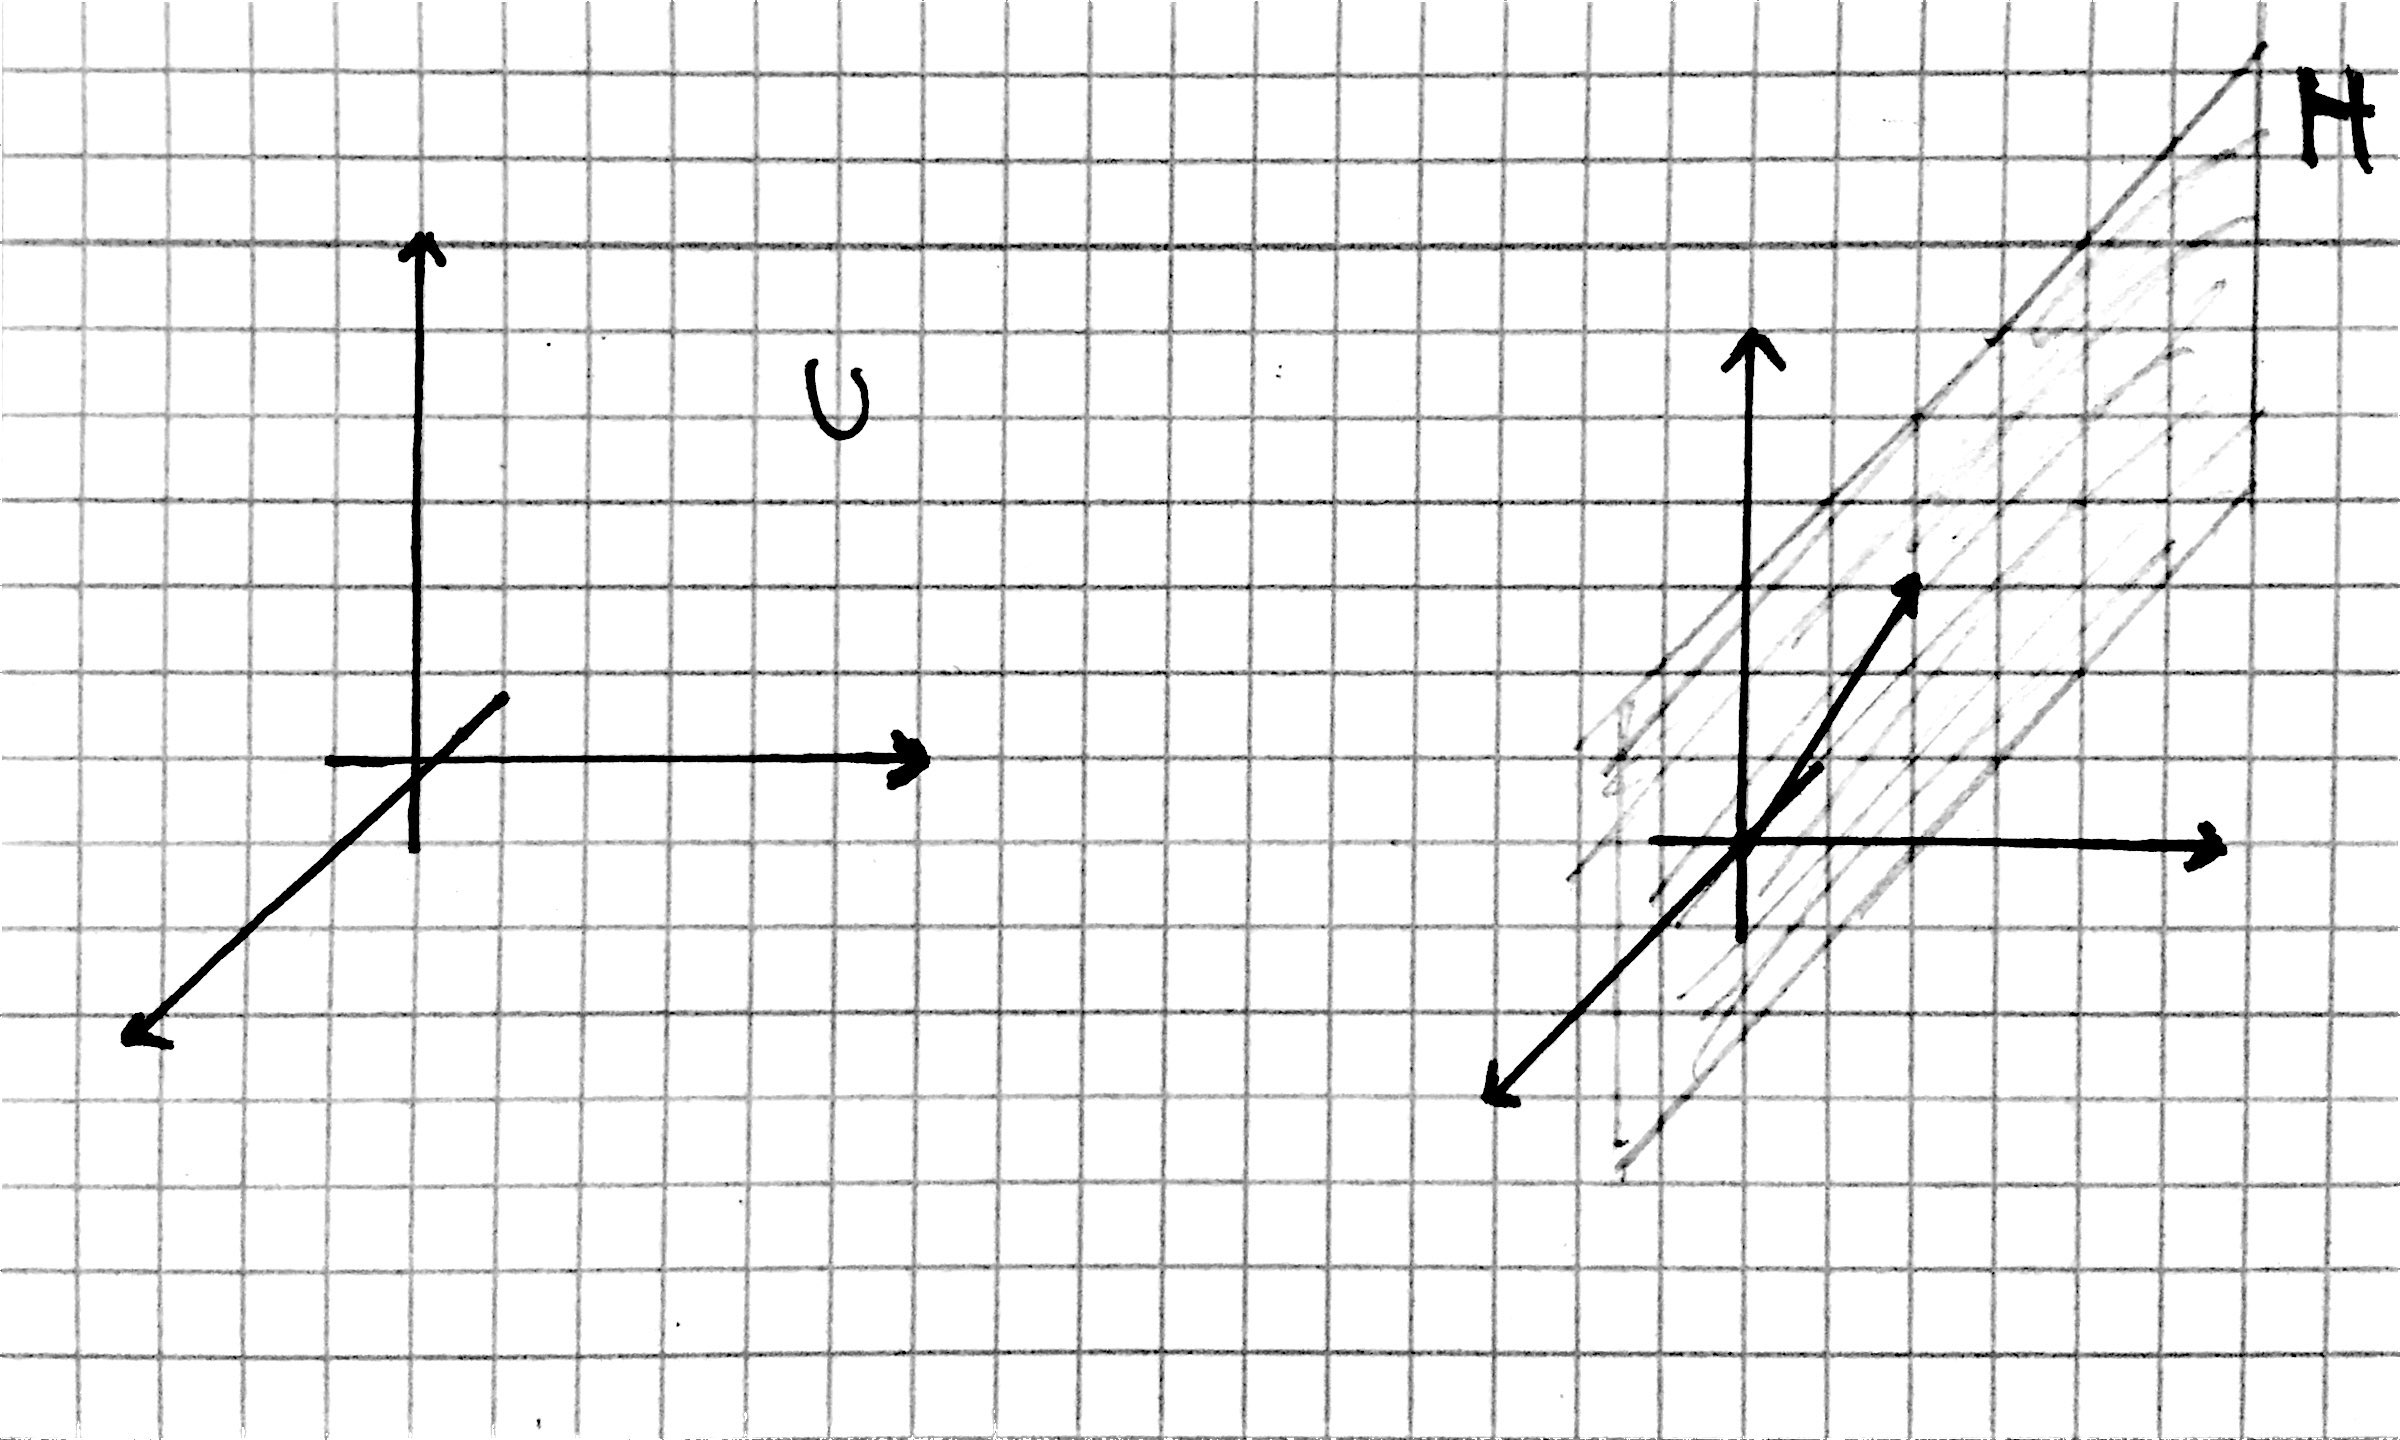
\includegraphics[scale=0.17]{la_1.jpg} 
 \section{Aufgabe 2}
 \subsection{i}
 $v_5 = v2+(-1)\cdot v_3 = (1,1,1,1)-(0,1,1,0)=(1,0,0,1)$ \checkmark \\
 $v_6 = v_2+v_3 = (1,1,1,1) + (0,1,1,0) = (1,2,2,1)$ \checkmark \\
 \subsection{ii}
 Zu zeigen ist: $span(\{v_2,v_5,v_6\}) = span(\{v_3,v_5,v_6\}) $\\
 Wir suchen die Basis der beiden Vektorräume und vergleichen dann diese um deren Gleichheit zu prüfen.\\
 Wir schreiben die Vektoren in eine Matrix und bringen diese in norm. ZSF um die linear unabhängige Vektoren zu finden.\\
 \begin{equation*}
 \begin{pmatrix}
 1&1&1&1 \\ 1&0&0&1 \\ 1&2&2&1
 \end{pmatrix} \Rightarrow
 \begin{pmatrix}
 0&1&1&0 \\ 1&0&0&1 \\ 1&2&2&1
 \end{pmatrix} \Rightarrow
 \begin{pmatrix}
 0&1&1&0 \\ 1&0&0&1 \\ 1&0&0&1
 \end{pmatrix} \Rightarrow
 \begin{pmatrix}
 0&1&1&0 \\ 1&0&0&1 \\ 0&0&0&0
 \end{pmatrix}
 \end{equation*}
 Daraus folgt, $basis( span(\{v_2,v_5,v_6\}) = \{(0,1,1,0),(1,0,0,1) \}$\\
 \begin{equation*}
 \begin{pmatrix}
   0&1&1&0 \\ 1&0&0&1 \\ 1&2&2&1
 \end{pmatrix} \Rightarrow
 \begin{pmatrix}
   0&1&1&0 \\ 1&0&0&1 \\ 1&1&1&1
 \end{pmatrix} \Rightarrow
 \begin{pmatrix}
   0&1&1&0 \\ 1&0&0&1 \\ 0&1&1&0
 \end{pmatrix} \Rightarrow
 \begin{pmatrix}
   0&1&1&0 \\ 1&0&0&1 \\ 0&0&0&0
 \end{pmatrix} 
 \end{equation*}
 Daraus folgt, $basis(span(\{v_3,v_5,v_6\})) = \{(0,1,1,0),(1,0,0,1) \}$\\
 Da die zwei Vektorräume die gleiche Basis haben können wir sagen, dass die zwei Vektorräume gleich sind.
 \subsection{iii}
 \begin{equation*}
 \begin{pmatrix}
 1&2&1&2 \\ 1&1&1&1 \\ 0&1&1&0 \\ 0&1&0&1 \\ 1&0&0&1 \\ 1&2&2&1 
 \end{pmatrix} \Rightarrow
 \begin{pmatrix}
 0&1&0&1 \\ 1&1&1&1 \\ 0&1&1&0 \\ 0&1&0&1 \\ 1&0&0&1 \\ 1&1&1&1 
 \end{pmatrix} \Rightarrow
 \begin{pmatrix}
 0&1&0&1 \\ 1&1&1&1 \\ 0&1&1&0 \\ 0&0&0&0 \\ 1&0&0&1 \\ 0&0&0&0 
 \end{pmatrix} \Rightarrow
 \begin{pmatrix}
 0&1&0&1 \\ 0&1&1&0 \\ 0&1&1&0 \\ 0&0&0&0 \\ 1&0&0&1 \\ 0&0&0&0 
 \end{pmatrix} \Rightarrow
 \begin{pmatrix}
 0&1&0&1 \\ 0&1&1&0 \\ 1&0&0&1 \\ 0&0&0&0 \\ 0&0&0&0 \\ 0&0&0&0 
 \end{pmatrix} 
 \end{equation*}
 Also ist basis($span(\{v_1,v_2,v_3,v_4,v_5,v_6\}) $) = $ \{(0,1,0,1),(0,1,1,0),(1,0,0,1)\} $\\
 Sei B =  $ \{(0,1,0,1),(0,1,1,0),(1,0,0,1)\} $ dann ist B linear unabhängig und $B \subseteq S$,\\
 span(B) = span(S) da B das minimale Ereugungendensystem von S ist.
 \section{Aufgabe 3}
 \subsection{i}
 Seien die Vektoren $s_1, ... , s_n \in S$ linear abhängig mit $S \subseteq V$ ,dann gibt es koeffizienten $\lambda_1 , ... , \lambda_n \in \mathbb{K}$ für die gilt $\lambda_1 s_q + ... + \lambda_n s_n = 0$.\\
 Daraus folgt $0 = \phi(0) = \phi(\lambda_1 s_q + ... + \lambda_n s_n) = \lambda \phi(s_1)+...+\lambda \phi(s_n)$\\
 Also sind $ \phi(s_1),...,\phi(s_n)$ linear abhängig.
 \subsection{ii}
 \section{Aufgabe 4}
 \subsection{i}
 Sei $\{\phi(b_1),...,\phi(b_n)\} \text{ ein Erzeugendensystem von W } \Rightarrow \text{ ist } \phi $ offenbar surjektiv, da alle Vektoren aus W als kombination der Urbilder von $\phi(b_1),...,\phi(b_n)$ darstellbar sind.\\
 $\text{Sei ein Vektor } c \in W \text{ und die Koeffizienten } a_1,...,a_n \in K \Rightarrow \\ c = a_1\phi(b_1)+...+a_n\phi(b_n) \underset{\phi Homomorphismus}{=} \phi(a_1 b_1)+...+\phi(a_n b_n)\\ $\\
 $ \underset{\phi Homomorphismus}{=} \phi(a_1 b_1+...+a_n b_n) $ \\
 Also hat $\phi$ immer eine lösung und ist somit Surjektiv.
 \subsection{ii}
 $\{b_1,...,b_n \}$ sind nach aufgabendefinition eine linear unabhängige Teilmenge von V $\Rightarrow$  Seien $a_1,...,a_n \in K$ ist die einzige Lösung für die Gleichung:\\ $a_1b_1+...+a_nb_n=0$ die triviale mit $a_1=...=a_n = 0$.\\
 $\Rightarrow 0=a_1b_1+...+a_nb_n \underset{\phi \text{ injektiv und Homomorhismus}}{=} a_1\phi(b_1)+...+a_n\phi(b_n)$\\
 Also da $\phi$ injektiv ist die menge $\{\phi(b_1),...,\phi(b_n)\}$ linear unabhängig.
 \subsection{iii}
 Sei $b := (b_1, ...,b_n) \in K^m$ und $A:=\alpha_{ij} \in K^{m\times n}$ mit $1\leq i\leq m \text{ und } 1\leq j \leq n$, $m,n \in \mathbb{N}$ gibt es ein LGS der Form: \\
 $ \alpha_{11}a_1+...+ \alpha_{1n}a_n = b_1 $\\
 $ \vdots \;\;\;\;\;\;\;\;\;\;\;\;\;\;\;\;\;\;\;\;\;\;\;\;  \vdots$ \\
 $ \alpha_{m1}a_1+...+ \alpha_{mn}a_n = b_m $\\
 Das kann auch in Form einer Matrix geschrieben werden:
 $$ 
 \begin{pmatrix}
	\alpha_{11}a_1 && \dotsb && \alpha_{1n}a_n \\ \vdots && && \vdots \\ \alpha_{m1}a_1 && \dotsb && \alpha_{mn}a_n 
 \end{pmatrix} 
 \begin{pmatrix}
	a_1 \\ \vdots \\ a_n 
 \end{pmatrix} =
 \begin{pmatrix}
	b_1 \\ \vdots \\ b_m
 \end{pmatrix} 
 $$
 Da die Vektoren $\{ a_1, .. a_n\}$ teil eines Erzeugendensystem von $K^m$ sind, können wir annehmen, dass $\forall b \in K^m \; \exists A \in K^{m\times n} : Ax=b, \; x \in \{a_1,...,a_n\}$.
 Das wollten wir nämlich zeigen, für alle b aus $K^m$ existiert immer mindestens eine Lösung für die Gleichung $Ax = b$, eine lineare kombination aus mehrfachen der Elemente der Vektoren aus dem erzeugenden System von $K^m$.
 \subsection{iv}
 Aus der Aufgabendefinition ist klar ersichtlich, dass sei $x \in K^n$ und  $A:=\alpha_{ij} \in K^{m\times n}$ gibt es ausschliesslich die triviale Lösung für den folgenden LGS:\\
 $ \alpha_{11}x_1+...+ \alpha_{1n}x_n = 0 $\\
 $ \vdots \;\;\;\;\;\;\;\;\;\;\;\;\;\;\;\;\;\;\;\;\;\;\;\;  \vdots\;\;\;\;\;\;\;\;\;\;\;\;\;\;\;\;\;\;\;\;\;\;\;\; \Rightarrow \text{ ist nur durch } x = 0 \text{ lösbar}$ \\
 $ \alpha_{m1}x_1+...+ \alpha_{mn}x_n = 0 $\\
 Daraus lässt sich erschliessen, dass für den analogen fall $A\begin{pmatrix} x_1 \\ \vdots \\ x_n \end{pmatrix} = \begin{pmatrix} a_1 \\ \vdots \\ a_m \end{pmatrix}$ das gleiche gilt. \\ 
 Und da $0_m$ nicht durch einer linearen Kombination aus $\{a_1, ... , a_n\}$ darstellbar ist. Folgt, dass die Menge $\{a_1, ... , a_n\} \subseteq \mathbb{R}^n$  linear unabhängig ist.
\end{document}